\renewcommand{\chaptername}{} % remove "Capítulo"
\chapter{FUNDAMENTAÇÃO TEÓRICA}  %Capitulo 3
%\addcontentsline{toc}{chapter}{FUNDAMENTAÇÃO TEÓRICA}

Neste Capítulo é apresentada a fundamentação teórica dos principais conceitos relacionados à análise de desempenho e à eficiência energética de usinas fotovoltaicas. Na Seção 3.1 é discutido sobre geração distribuida, na Seção 3.2 é discutido acerca carport solar e na Seção 3.3 é discutido acerca os principais índices de desempenho.


\section{GERAÇÃO DISTRIBUIDA}

Na geração distribuída, os microinversores são comumente utilizados para realizar o monitoramento da geração de energia em sistemas de pequeno e médio porte. Os microinversores, em particular, têm ganhado espaço por permitir o rastreamento individualizado do Ponto de Máxima Potência (MPPT) por módulo, mitigando as perdas por sombreamento parcial e por incompatibilidade (PARENTE, 2021), que são fatores críticos para a eficiência neste tipo de estrutura.

\section{CARPORT SOLAR}

O carport é uma estrutura metálica, que serve como cobertura para áreas de estacionamento, com os painéis fotovoltaicos instalados em seu telhado inclinado. As estruturas carport aproveitam espaços já construídos, como estacionamentos, para integrar a geração fotovoltaica, oferecendo sombreamento e, frequentemente, servindo como ponto de recarga para veículos elétricos (KULIK, 2024).

\section{ÍNDICES DE DESEMPENHO}

Para avaliar a viabilidade e o desempenho dessas instalações, são utilizados indicadores chave de desempenho (KPIs). Os KPIs são fundamentais para identificação de falhas (REDISKE et al., 2024). Dentre os KPIs mais relevantes, destacam-se a Produtividade Final (Yf), o Fator de Capacidade (CUF) e a Taxa de Desempenho (PR). Estes índices permitem diagnosticar a qualidade da conversão da energia solar em elétrica, identificar perdas operacionais, e comparar o desempenho de sistemas em diferentes localidades e com distintas tecnologias.

Os indicadores chave de desempenho (KPIs) desse trabalho estão descritos a seguir:
\newpage

\textbf{a. Taxa de  Desempenho (PR)}
\newline


A taxa de desempenho é um importante indicador para apontar a eficiência geral do sistema fotovoltaico em relação a incidência de irradiação (PARENTE, 2021). Esse KPI consiste na divisão entre a produtividade final (Yf) e o rendimento de referência (Yr) que é dado pela divisão entre a irradiância no plano do módulo em kW/m² (Ht) e a irradiância de referência (G) no valor de 1kW/m² (REDISKE et al., 2024). Assim sua equação é dada por: 


\begin{center}
    $ PR = \frac{Y_f \cdot G}{H_t}$
\end{center}
    



Os valores de irradiância no plano do módulo (Ht) para a cidade de São Cristóvão, onde está localizado o Sergipe Parque Tecnológico - SergipeTec, foram coletados mensalmente através do Centro de Referência para as Energias Solar e Eólica Sérgio de S. Brito (CRESESB,2025) utilizando os dados de latitude e longitude colocados no programa SunData.
\newline

\textbf{b.	Fator de Utilização de Capacidade (CUF)}
\newline

O fator de utilização de capacidade é definido como a razão entre a produção anual real de energia e a quantidade de energia que a usina solar fotovoltaica geraria se fosse operada na potência nominal máxima por 24 horas por dia durante um ano (REDISKE et al., 2024). Assim sua equação é dada por:

\begin{center}
    $ 24h \cdot 365d = 8760$ \\
    $CUF = \frac{Y_f}{8760} = \frac{E_{pv}}{P_{nom} \cdot 8760}$
\end{center}

Sendo a potência dos módulos fotovoltaicos conectados ao seu respectivo microinversor como a potência nominal utilizada.
\newline

\textbf{c.	Rendimento Final ou Produtividade ($Y_f$)}
\newline

A produtividade final é um indicador bastante disseminado no mercado de energia fotovoltaico devido a sua objetividade, pois permite uma comparação justa entre sistemas que possuem potências ou áreas diferentes (PARENTE, 2021). Esse KPI indica o número de horas necessárias para que o conjunto fotovoltaico opere em sua potência nominal para fornecer a mesma energia (REDISKE et al., 2024). Além disso, consiste na divisão entre a energia CA gerada pelo sistema (kWh) e a potência nominal dos módulos fotovoltaicos (kW). Assim sua equação é dada por: 

\begin{center}
    $Y_f = \frac{E_{ca}}{P_{nom}}$
\end{center}
\newline

\textbf{d.	Rendimento ou Produtividade do Arranjo ($Y_a$)}
\newline

Esse KPI indica o número de horas necessárias para operar o sistema em sua capacidade nominal de geração de energia real, sendo responsável por avaliar o desempenho em corrente contínua (DC) do sistema fotovoltaico (REDISKE et al., 2024). A sua equação é dada por: 

\begin{center}
    $Y_a = \frac{E_{cc}}{P_{nom}}$
\end{center}

Sendo $E_cc= \frac{E_{ca}}{0,95}$ e 0,95 sendo o valor da eficiência CEC do microinversor Deye modelo SUN2000G3-US-220 que é um parâmetro utilizado para quantificar o verdadeiro desempenho de um microinversor.
\newline

\textbf{e. Perdas (Pc e Ps)}
\newline

As perdas de captura é um KPI que indica as perdas devido à operação dos módulos fotovoltaicos, indicando o número de horas em que o sistema não captou a irradiação total (REDISKE et al., 2024). Essas perdas podem ser de dois tipos: as perdas por captura térmica são causadas quando a temperatura do painel fotovoltaico está acima de 25°C, já as perdas por captura diversas são causadas por problemas de fiação, sombreamento parcial, sujeiras, baixa irradicação e erros no MPPT (YALAWAR et al., 2018). Sua equação é dada por: 

\begin{center}
    $ P_c = Y_r - Y_a$
\end{center}

Já as perdas de sistema é um outro KPI que indica as perdas que ocorrem no restante do sistema fotovoltaico durante o processo de transmissão de eletricidade, indicando o número de horas que o sistema perdeu durante a conversão de energia CC para CA por causa da condução e elementos passivos do circuito elétrico (REDISKE et. al, 2024). Sua equação é dada por: 

\begin{center}
    $ 24h \cdot 365d = 8760$ \\
    $P_s = Y_a - Y_f$
\end{center}
\newline

\textbf{f.	Eficiência Global do Sistema (Egs)}
\newline

A Eficiência global do sistema indica a porcentagem de eficiência do sistema em converter energia solar em energia elétrica. Esse KPI consiste na divisão entre a energia elétrica gerada pelo sistema e o produto da área da usina pela irradiação solar média ao longo do período de estudo considerado. Asssim, sua equação é dada por: 

\begin{center}
    $ 24h \cdot 365d = 8760$ \\
    $E_{gs} = \frac{E_{el}}{A \cdot H_t}$
\end{center}

Sendo $E_{el}$ a energia gerada pelo sistema kWh, Ht a irradiância no plano do módulo em $kW/m^2$ e A a área dos módulos que compõe o sistema. 

Na Tabela \ref{fig:tab3} apresenta a relação dos principais KPIs utilizados neste trabalho, bem como a finalidade, os cálculos empregados conforme os artigos cientificos e as legendas com as identificações de cada elemento.


%\clearpage
\begin{table}[H]
    \centering
    \caption{\centering Indicadores chave de desempenho (KPIs)}
    \label{fig:tab3}
    \includegraphics[width=\textwidth]{Figuras/Indicadores Chave de Desempenho.pdf}

    {\fontsize{10pt}{12pt}\selectfont
    \textbf{Fonte:} Próprio Autor, 2025.}
\end{table}


Esses 7 KPIs listados acima são de extrema importância para comparar e analisar o desempenho dos 53 microinversores presentes na usina a fim de detectar falhas ou mau funcionamento em alguma operação.

\section{OPERAÇÃO E MANUTENÇÃO}

Em todo o processo relacionado a equipamentos, infraestrutura e serviços, deve-se ter práticas e atividades para garantir a melhor operação possível, atentando aos parâmetros de funcionamento do equipamento e prevendo as manutenções necessárias para manter as características nominais dos mesmos.

Trazendo para a geração fotovoltaica, além do comissionamento e estudo da eficiência por meio de indicadores, em todas as outras etapas de desenvolvimento, desde o projeto até o momento em que o sistema se encontra gerando, deve haver todo um processo e rotina de O\&M, alguns desses só são necessárias no início, como é o caso da análise do impacto do sombreamento do local de interesse sobre o gerador fotovoltaico, para tanto podem ser utilizadas ferramentas de simulação (como é o caso do software PV*SOL), onde é feita a modelagem 3D do local, atentando-se aos objetos que possam fazer sombra, pois o sombreamento impacta diretamente na eficiência da geração de energia, com isso, para uma operação eficiente é de suma importância escolher um local adequado, que também implica numa melhor manutenibilidade, pois envolve a facilidade de acesso e análise das influências do meio.


\renewcommand{\chaptername}{} % remove "Capítulo"
\chapter{METODOLOGIA}   %Capitulo 4
%\addcontentsline{toc}{chapter}{METODOLOGIA}
\label{cap:metodologia}

Neste Capítulo é apresentado a metodologia da proposta para analisar o desempenho e a eficiência energética da usina fotovoltaica instalada e certificar a confiabilidade do sistema. Além do cumprimento dos objetivos do trabalho e o cronograma das atividades.  



Dessa forma, para garantir o desenvolvimento e a confiabilidade do presente trabalho, a metodologia foi dividida em seções. Na Seção 4.1 é discutido sobre caracterização da pesquisa, na Seção 4.2 caracterização do sistema fotovoltaico, na Seção 4.3 é discutido sobre procedimento de coleta e tratamento de dados, na Seção 4.4 acerca de cálculo dos índices de performace e análise dos resultados;, e na Seção 4.5. é discutido sobre o diagrama de blocos do projeto. CORRIGIR


\section{CARACTERIZAÇÃO DA PESQUISA}

A natureza do estudo é do tipo quantitativa e exploratória, que compreende o levantamento da literatura existente sobre o desenvolvimento de estudo para análise de desempenho e eficiência energética de usinas fotovoltaicas. Esta etapa consiste em levantamento do material a partir de livros, artigos científicos, periódicos, datasheet dos equipamentos instalados, tutoriais, definições de parâmetros utilizados e delineação do projeto.  

Para Lakatos; Marconi (2009b, p. 269) quanto à abordagem (tratamento) dos dados, uma pesquisa pode ser quantitativa, qualitativa e quantiqualitativa, nesse sentido, optou-se pela quantitativa: Por ser um estudo de caso que foi expresso através da coleta de dados, utilizando indicadores chave de desempenho (KPIs) e exploratório realizado por meio de levantamento bibliográfico necessário para conhecimento.

Inicialmente fez-se uma revisão bibliográfica sobre os Indicadores chave de desempenho (KPIs), com foco em usinas solares. Essa etapa é essencial para a análise dos dados proveniente da usina instalada no Sergipe Parque Tecnológico (SergipeTec).



\section{CARACTERIZAÇÃO DO SISTEMA FOTOVOLTAICO}

CORRIGIR TEXTO:Inicialmente realizou-se um estudo de referencial teórico e revisão bibliográfica acerca de usinas solares carport, usina solares com microinversores e indicadores chave de desempenho (KPIs). Em seguida, efetuou-se o mapeamento da usina de carport solar com os 53 microinversores e 210 módulos fotovoltaicos que são conectados em cada microinversor, mapeamento completo encontra-se apresentado no \hyperref[ap:catalogacao-u]{APÊNDICE 1}. Em conjunto com essa atividade, realizou-se a coleta de dados gerais da usina solar em um intervalo de 1 ano, entre janeiro e dezembro de 2025, contendo as informações de energia produzida (kWh), potência (kW), tensão (V) e corrente (A) de todos as placas solares e microinversores durante esse intervalo de tempo utilizando o software SOLARMAN Smart. Além disso, também verificou-se o monitoramento de forma online o funcionamento de cada módulo e microinversor da usina a fim de detectar possíveis erros e falhas no sistema.




Para a realização deste trabalho, analisou - se uma usina solar do tipo carport de minigeração distribuída, composta por 210 módulos fotovoltaicos e 53 microinversores. A usina está instalada no estacionamento do Sergipe Parque Tecnológico - SergipeTec, localizado no município de São Cristóvão–SE. Foram utilizados dados completos de geração referentes a um período de um ano, compreendido entre janeiro e dezembro de 2025. Os dados da usina analisada foram disponibilizados e monitorados por meio de duas plataformas: SolarView e SOLARMAN Smart.

Um dos componentes do carport solar é a estrutura de longarinas em aço destinada à sustentação dos módulos fotovoltaicos, configurada no modelo de garagem solar com duas vagas. Apresentado no \hyperref[ap:datasheet-carport]{ANEXO 1}
 o manual de instalação e o datasheet do carport solar. A Figura \ref{fig:estr} apresenta as dimensões da estrutura e alguns aspectos do modelo adotado. 


%\clearpage
\begin{figure}[h!]
    \centering
    \caption{Estrutura da usina solar modelo carport.}
    \label{fig:estr}
    \includegraphics[width=\textwidth]{Figuras/Estrutura Usina - fig.pdf}

    {\fontsize{10pt}{12pt}\selectfont
    \textbf{Fonte:} Manual de
instalação do carport solar}
\end{figure}

Esta estrutura conta com um sistema de calhas destinado ao escoamento da água da chuva entre os carports solares, além de uma fita de vedação fixada entre os módulos fotovoltaicos. Adicionalmente, há um fixador intermediário que se estende por todo o comprimento da fileira de módulos e os fixador final que serve para prender com segurança o painel solar à estrutura metálica nos pontos de extremidade.

O sistema da usina é composto por 14 carports solares, sendo que cada carport contém 15 módulos solares policristalinos modelo JKM575N-72HL4-V da fabricante Jinko Solar e possuem 575 Wp cada um, totalizando um sistema de 120,75 kWp. A instalação ainda inclui 53 microinversores modelo SUN2000G3-US-220 da fabricante Deye de 2 kW cada, totalizando um sistema de 106 kW com monitoramento integrado. 

Na Tabela \ref{fig:espmod} e Tabela \ref{fig:espmicro} são apresentadas as informações técnicas, nas condições padrão de teste (STC), dos módulos fotovoltaicos e dos microinversores utilizados respectivamente e a vista aérea da usina solar na Figura \ref{fig:fotousina}:



\begin{table}[H]
    \centering
    \caption{\centering Especificações dos módulos fotovoltaicos.}
    \label{fig:espmod}
    \includegraphics[width=\textwidth]{Figuras/Especificações Modulo - tab1.pdf}

    {\fontsize{10pt}{12pt}\selectfont
    \textbf{Fonte:} Datasheet Tiger Neo N-type 72HL4-(V) 570-590 Watt}
\end{table}

No \hyperref[ap:datasheet-modulos]{ANEXO 2} são apresentadas as características técnicas dos 210 módulos fotovoltaicos utilizados na usina solar do SergipeTec, com os dados obtidos do Datasheet Tiger Neo N-type 72HL4-(V) 570-590 Watt.

\begin{table}[H]
    \centering
    \caption{\centering Especificações dos microinversores}
    \label{fig:espmicro}
    \includegraphics[width=\textwidth]{Figuras/Especificações Microinversores - tab2.pdf}
    {\fontsize{10pt}{12pt}\selectfont
    \textbf{Fonte:} Datasheet MicroInversor SUN2000G3-US-220}
\end{table}

Já no \hyperref[ap:datasheet-microinversores]{ANEXO 3} são apresentadas as características técnicas dos 53 microinversores utilizados na usina solar do SergipeTec, com os dados obtidos do Datasheet MicroInversor SUN2000G3-US-220.

\begin{figure}[H]
    \centering
    \caption{\centering Usina solar modelo carport no estacionamento do SergipeTec}
    \label{fig:fotousina}
    \includegraphics[width=\textwidth]{Figuras/Usina Carport - fig2.pdf}
    {\fontsize{10pt}{12pt}\selectfont
    \textbf{Fonte:} Próprio Autor, 2025}
\end{figure}


Acima podemos ver a usina localizada no SergipeTec composta por 210 módulos fotovoltaicos divididos em 14 estruturas carport servindo para a geração de energia elétrica e também como um estacionamento sombreado para veículos.





\section{PROCEDIMENTO DE COLETA E TRATAMENTO DE DADOS}


Na etapa seguinte, efetuou-se os levantamentos dos dados coletados no monitoramento da usina, dos valores médios de irradiação solar obtidos pelo CRESESB e também das faturas de energia de todas as unidades consumidoras (UCs) presentes no SergipeTec. A partir daí serão utilizados diferentes programas e softwares para realização de cálculos e simulações. O Excel será utilizado para criação de planilhas contendo os cálculos dos KPIs de cada microinversor da usina e os cálculos de análise financeira e econômica, contendo os dados de retorno sobre o investimento e o tempo de retorno financeiro (payback) do sistema fotovoltaico. Já o software PV*SOL será utilizado para efetuar a análise do sombreamento sobre o gerador fotovoltaico e análise do retorno econômico quanto a eficiência do conjunto gerador, por meio de uma simulação 3D do gerador fotovoltaico, atentando-se aos objetos que possam vir a fazer sombra, agregando ao estudo da eficiência da inserção do gerador no local escolhido.

Em seguida, utilizando os programas Excel e Power BI serão gerados gráficos mostrando o resultado das informações mais importantes desse trabalho, como a comparação de desempenho dos KPIs entre cada um dos 53 microinversores, desempenho geral da usina com base no KPI da Taxa de Desempenho (PR) e também o gráfico de retorno financeiro, mostrando em quanto tempo a usina solar começa a ter um retorno financeiro positivo em relação ao valor investido para sua construção. Já utilizando o PV*SOL, após o final da simulação 3D de sombreamento da usina, será gerado um relatório de eficiência contendo informações acerca da eficiência da geração quanto a características técnicas e financeiras, mostrando também um prazo de amortização e eficiência do gerador ao longo dos anos com base no consumo anual médio estipulado.

Por fim, após a obtenção dos resultados acima, será necessário analisar o sistema fotovoltaico a fim de comparar o desempenho de cada microinversor, observar o efeito causado pelo sombreamento ao longo dos meses e avaliar a economia e o retorno financeiro referente à usina solar. A partir desses resultados será possível detectar falhas ou mau funcionamento da usina, seja por problemas em algum componente específico ou por conta de sombreamento elevado e também obter a projeção de quanto tempo falta para a usina abater o investimento para sua construção apenas com a economia nas faturas de energia.


\begin{comment}
    
    \captionsetup[figure]{name=Anexo} % muda o nome apenas para a próxima figura
    
    \begin{figure}[h!]
        \centering
        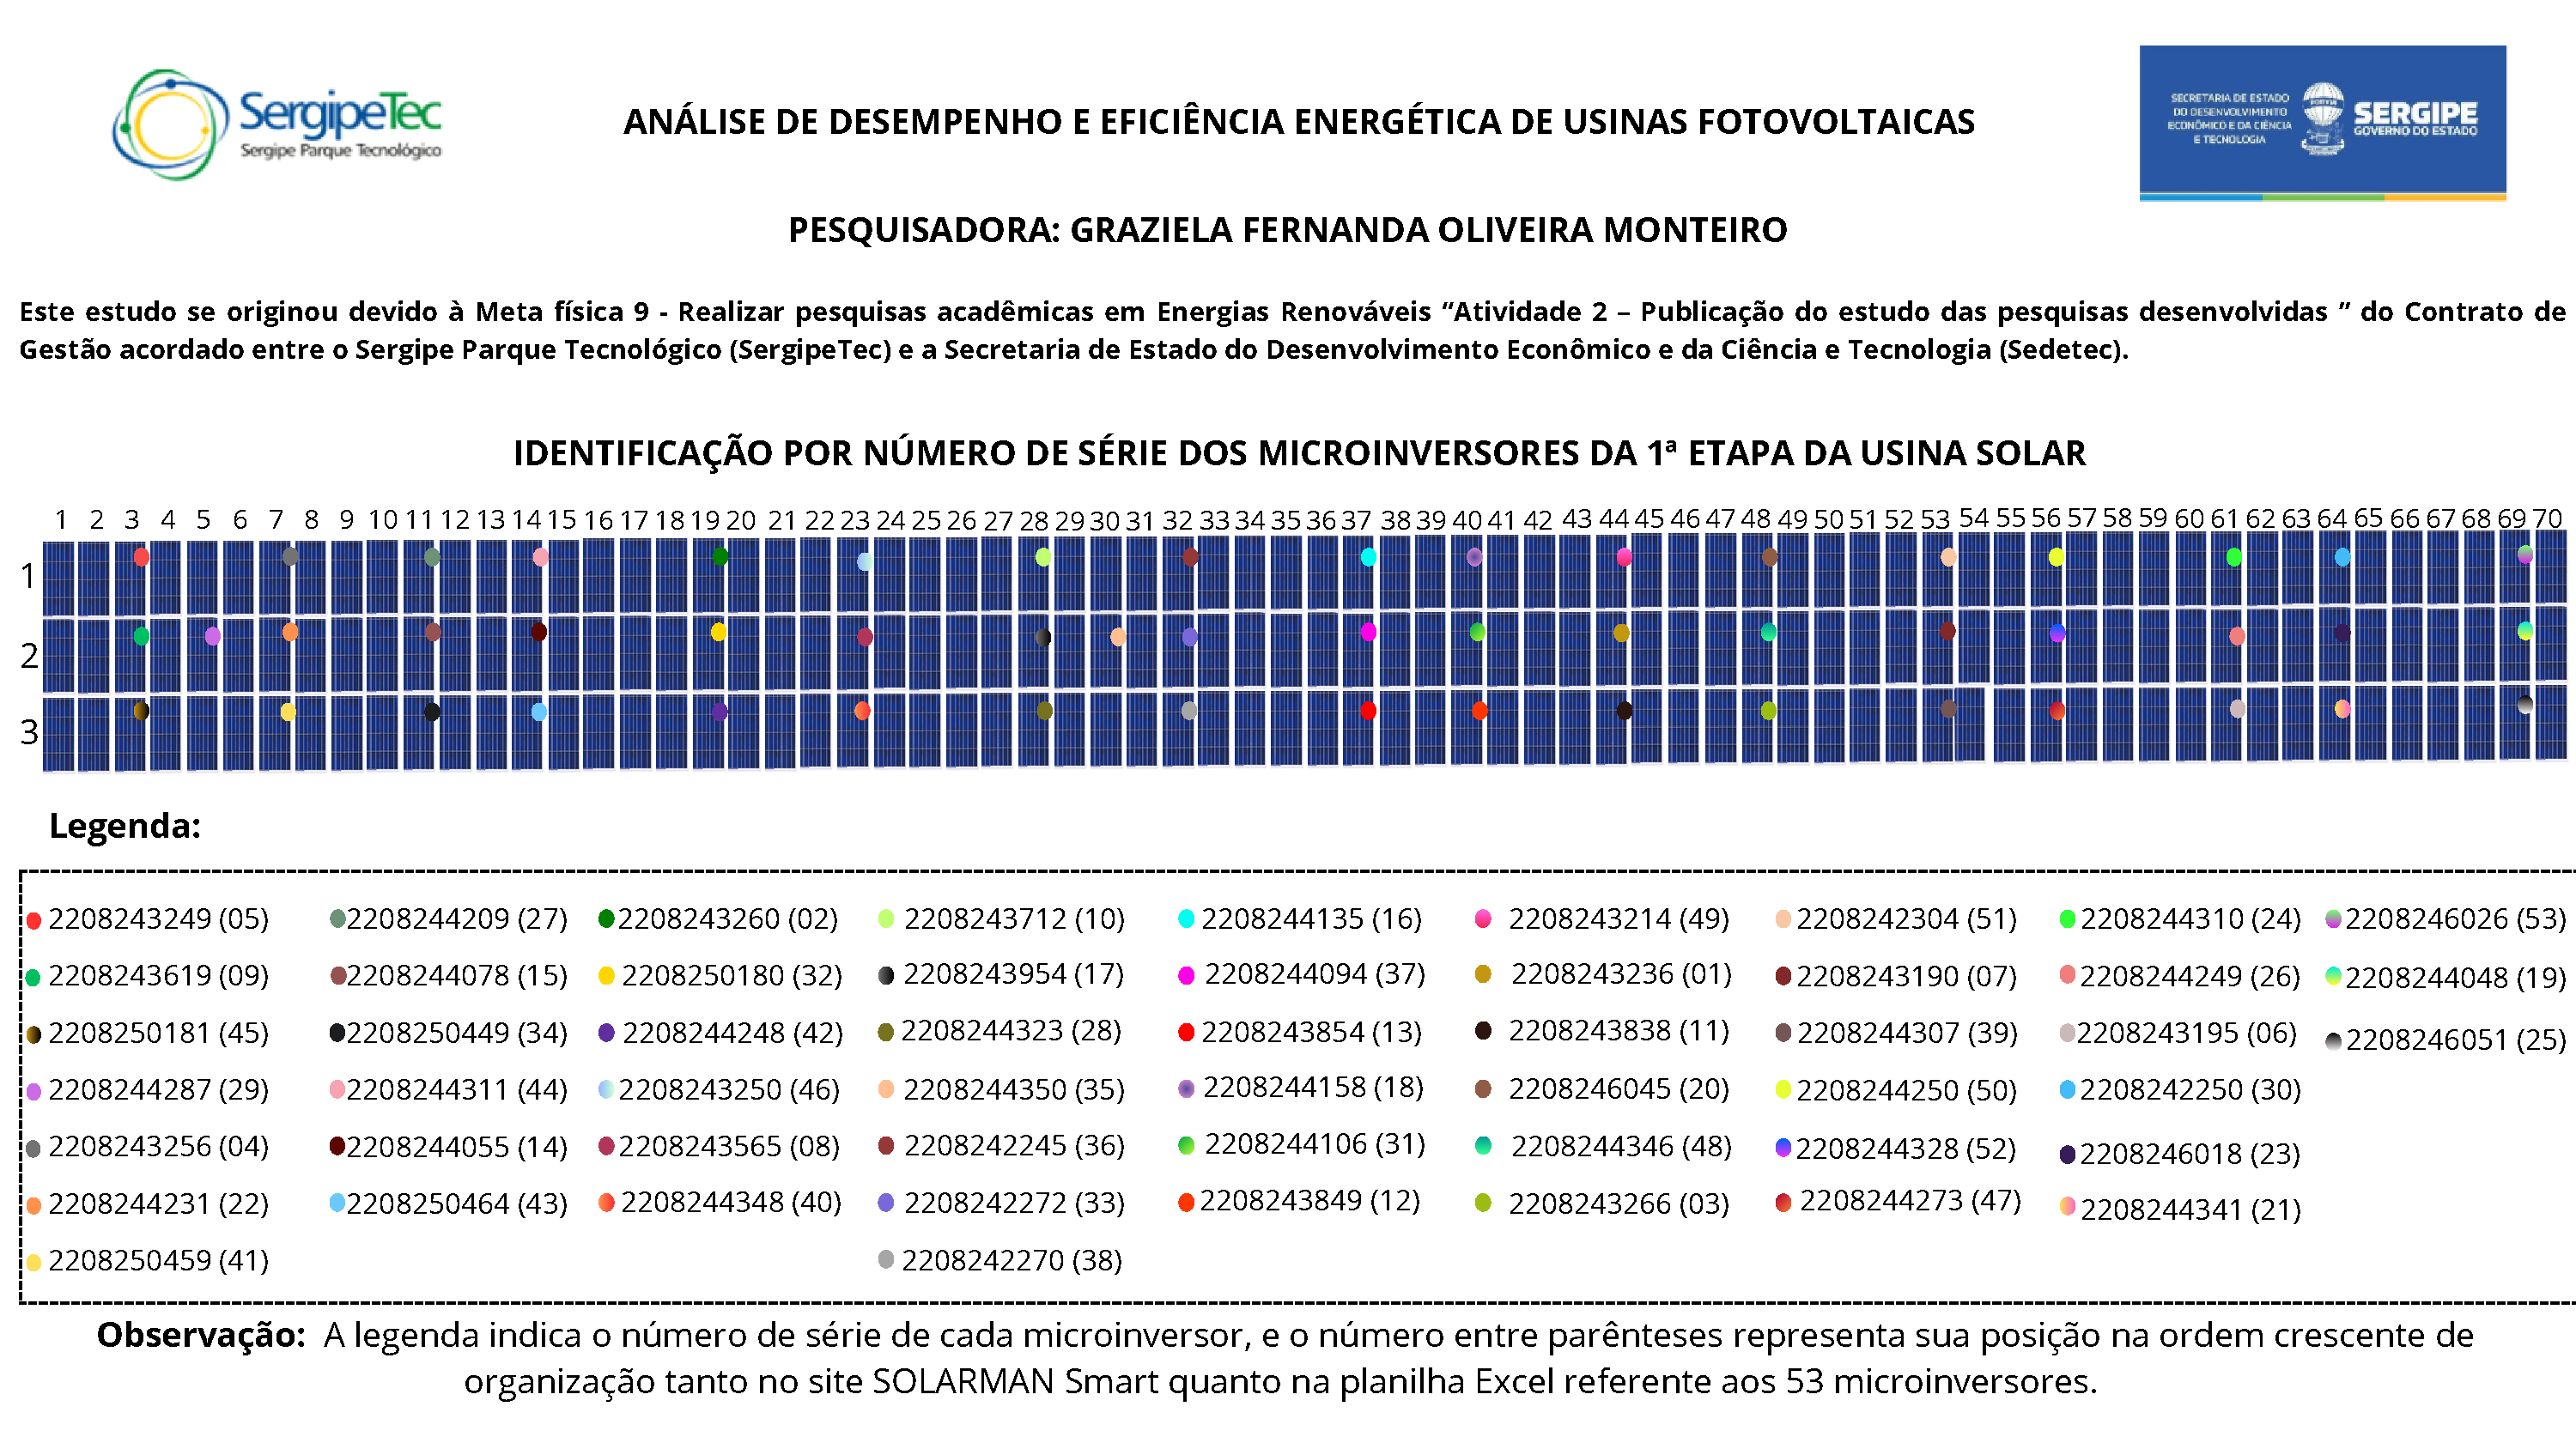
\includegraphics[page=1, width=\textwidth]{Anexos/CATALOGAÇÃO DA USINA SOLAR DO SERGIPETEC - 1ª ETAPA - GERAL.pdf}
        \caption{Exemplo de figura extraída do PDF — página 1}
        \label{fig:pdfpag1}
    \end{figure}
    
    % ---- restaurar o nome padrão ----
    \captionsetup[figure]{name=Figura}
    
    \begin{figure}[h!]
        \centering
        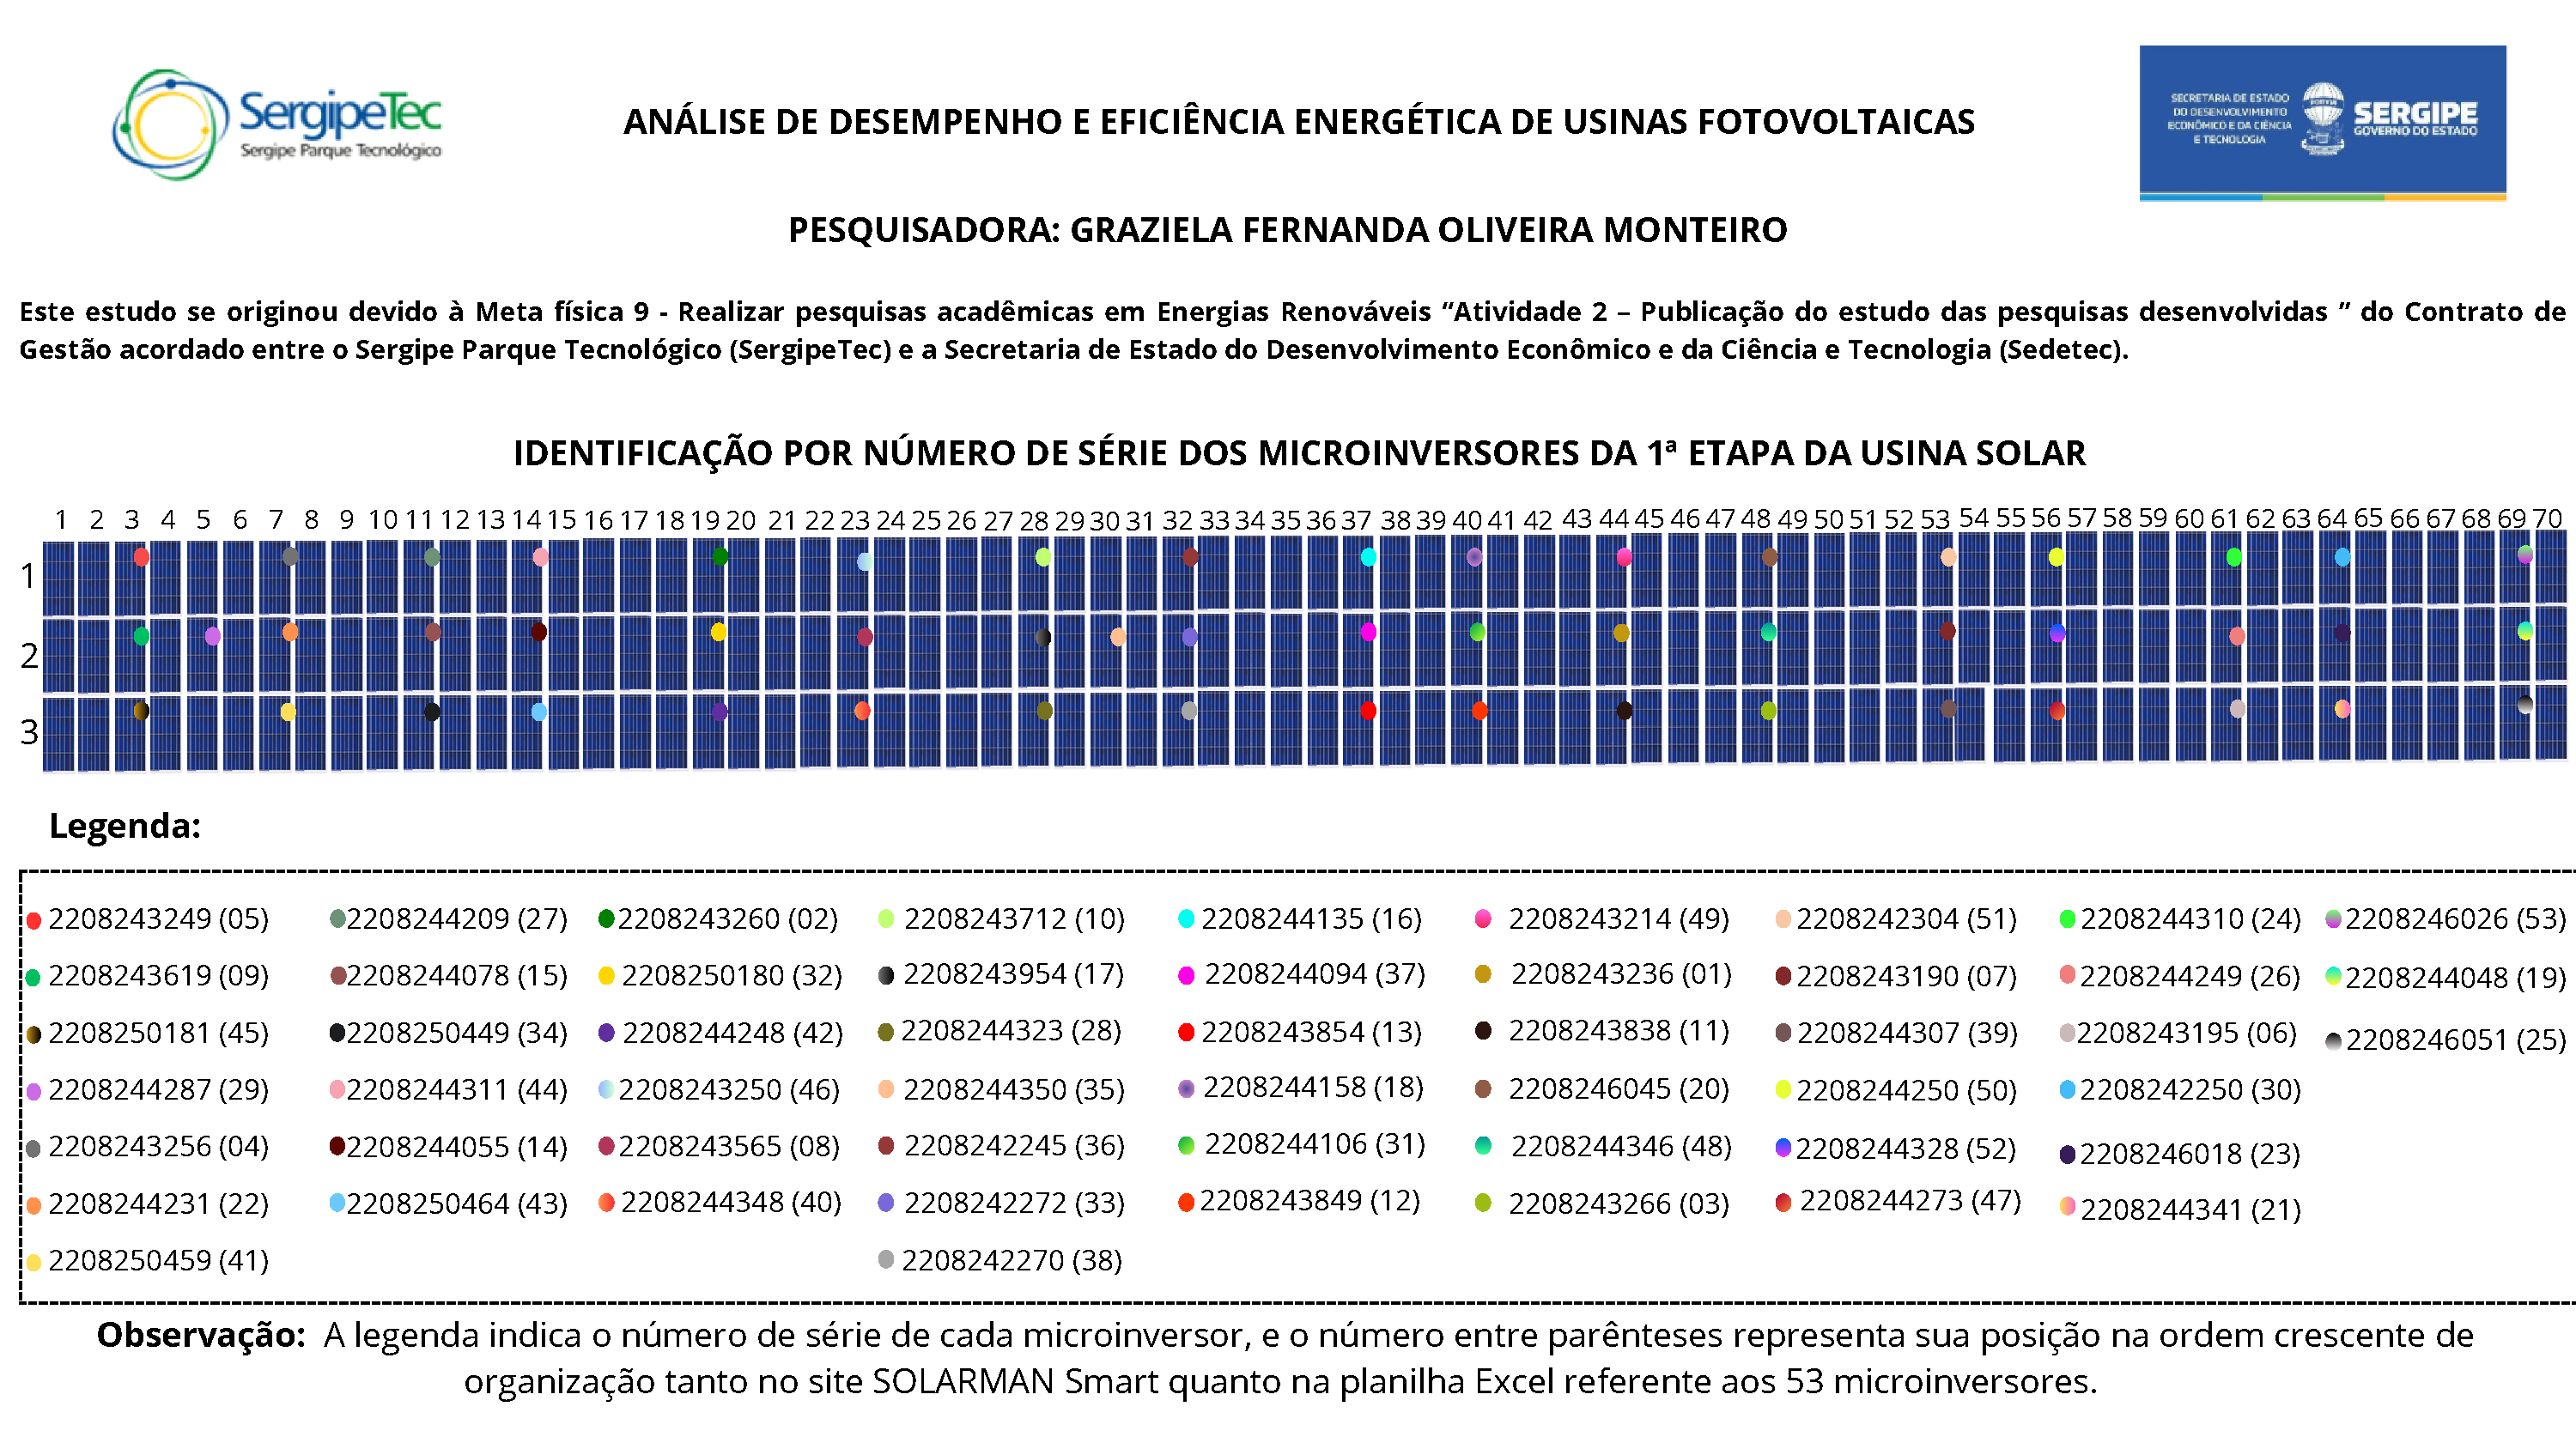
\includegraphics[page=1, width=0.9\textwidth]{Anexos/CATALOGAÇÃO DA USINA SOLAR DO SERGIPETEC - 1ª ETAPA - GERAL.pdf}
        \caption{Página 1 do PDF redimensionada}
        \label{fig:pdfpag2}
    \end{figure}

\end{comment}








\section{DIAGRAMA DE BLOCOS}

O diagrama de bloco mostra de forma simplificada toda a estrutura e os passos dessa dissertação, ilustrada na Figura 4.3: Diagrama de Blocos da Proposta de Dissertação.

\begin{figure}[H]
    \centering
    \caption{Diagrama de blocos da proposta de dissertação.}
    \includegraphics[width=5.0in]{Figuras/Fluxograma.pdf}
    \label{fig:Flux1}
    
    {\fontsize{10pt}{12pt}\selectfont
    \textbf{Fonte:} Próprio Autor, 2025}
\end{figure}


\renewcommand{\chaptername}{} % remove "Capítulo"
\chapter{RESULTADOS E DISCUSSÔES}
















 
\renewcommand{\chaptername}{} % remove "Capítulo"
\chapter{CRONOGRAMA DE ATIVIDADES}
%\addcontentsline{toc}{chapter}{CRONOGRAMA DE ATIVIDADES}

\label{sec:cronograma}
{\color{red}
O cronograma das atividades propostas para a realização deste trabalho é disposto na Figura \ref{fig:crono}, sendo elas:

\begin{itemize}
\justifying

    \item A1: Referencial teórico e revisão bibliográfica acerca de usinas solares carport, usina solares com microinversores e indicadores chave de desempenho (KPIs);
    \item A2: Mapeamento da usina de carport solar;
    \item A3: Monitoramento da usina e coleta de dados de geração via Solarman Smart;
    \item A4: Estudo da fundamentação teórica sobre indicadores chave de desempenho (KPIs);
    \item A5: Levantamento dos dados dos indicadores chave de desempenho (KPIs) em planilha Excel, preparação para cálculos de KPIs;
    \item A6: Cálculos dos indicadores chave de desempenho (KPIs), cálculo de payback e economia anual;
    \item A7: Levantamento das faturas de energia, através da coleta de informações durante um período de 1 ano antes e 1 ano após a primeira etapa da usina; 
    \item A8: Simulação de sombreamento (PV*SOL), modelagem 3D da usina, análise de sombreamento e impacto no desempenho;
    \item A9: Levantamento bibliográfico sobre energia solar, sombreamento, microinversores, KPIs, análises financeiras, usinas fotovoltaicas; 
    \item A10: Análise financeira e econômica, geração de gráficos de desempenho, KPIs por microinversor, gráficos financeiros (payback);
    \item A11: Geração de gráficos de KPIs (Excel e Power BI) e gráficos de retorno financeiro;
    \item A12: Relatório de eficiência; consolidação dos resultados técnicos e financeiros, análise final da usina;
    \item A13: Escrita da dissertação;
    \item A14: Defesa de dissertação.

\end{itemize}
}

%mudar a defesa para fevereiro
%empurrar a redacao do artigo para frente

\begin{figure}[H]
    \centering
    \caption{Cronograma de atividades previstas.}
    \label{fig:crono}
    \includegraphics[width=\textwidth]{Figuras/cronograma de atividades.pdf}
    
    {\fontsize{10pt}{12pt}\selectfont
    \textbf{Fonte:} Próprio Autor, 2025}
\end{figure}




 